\section{Nozioni generali su HEC-RAS e sul suo utilizzo}
HEC-RAS è un programma di modellazione idraulica, utilizzato per studiare il flusso d'acqua nei canali naturali o non.\\
Tale programma è stato prodotto dal Genio Militare Americano, venendo liberamente rilasciato nel 1995 \cite{hec-ras}.\\
Essendo un programma di simulazione, HEC-RAS permette di svolgere ``what-if scenario", ovvero valutazioni predittive, in merito ad eventi di deflusso estremo o ad inserimento in alveo di particolari opere; tale applicazione è coerente con il lavoro effettuato in questa relazione, ovvero la valutazione delle aree di inondazione per un certo evento di piena.\\
Al fine di poter compiere una simulazione idraulica è necessario che vengano definiti ed impostati alcuni parametri, tra i quali:
\begin{itemize}
    \item spaziali: come per esempio il dominio di calcolo (ovvero alveo e zone inondabili);
    \item condizioni al contorno: ovvero la portata entrante nel dominio di calcolo e le caratteristiche del tratto uscente;
    \item scabrezza del letto del fiume e delle aree inondabili (coefficiente di Manning);
    \item corpi naturali/artificiali presenti in alveo (come per esempio piloni di ponti o arginature).
\end{itemize}

\subsection{Sistema di calcolo}

Tutti i parametri precedentemente elencati sono strettamente collegati con la mesh, ovvero il reticolo di calcolo: mediante tale suddivisione (in elementi finiti come linee o poligoni) il programma svolge i calcoli di modellazione idraulica \cite{grid_and_dual_grid}.\\
La grandezza delle singole celle della griglia regola il numero di calcoli che il programma deve svolgere, con una conseguente variazione del tempo di processamento. Ovviamente, il tempo di calcolo e la bontà del risultato sono due fattori inversamente proporzionali rispetto alla grandezza delle celle di calcolo.\\
Teoricamente, sarebbe possibile imporre una mesh di calcolo a maglie estremamente piccole, in modo da rendere la simulazione più affidabile, purtroppo questa ipotesi renderebbe il processo globalmente meno efficiente.\\
Affinché sia possibile applicare i principali algoritmi di analisi, ad ogni cella della mesh è possibile associare un relativo valore di scabrezza, che varia in base alla tipologia di superficie indicata (come per esempio arginature o tratti in roccia).\\
Al fine di rendere più realistico il risultato finale, è possibile imporre delle linee (breaklines) dove far aderire meglio la mesh al suolo, cambiando la disposizione del reticolo o la sua grandezza; per esempio, in prossimità delle arginature o nel caso di soglie in alveo \eqref{figure:particolare_mesh}.

\begin{figure}[htb] \centering
    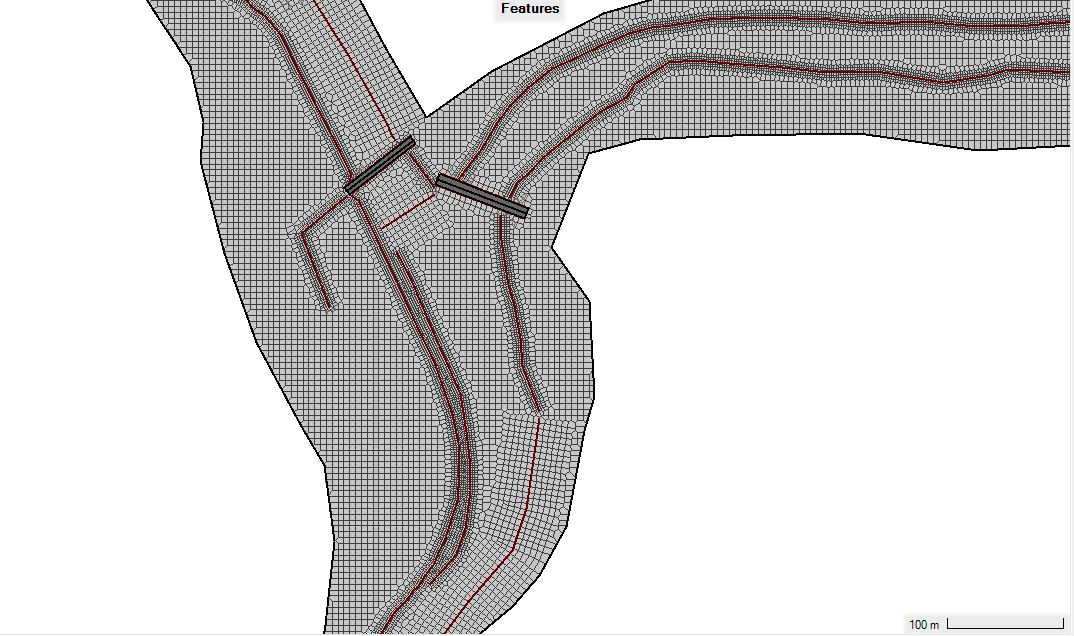
\includegraphics[scale=0.4]{immagini/particolare_mesh.JPG}
    \caption{Frazione della mesh del tratto di studio analizzato.}
    \label{figure:particolare_mesh}
\end{figure}

Il software ricava i parametri del suolo dal file DTM (digital terrain model) della relativa area di studio, precedentemente caricato dall'utilizzatore \eqref{figure:particolare_dtm}.

\begin{figure}[htb] \centering
    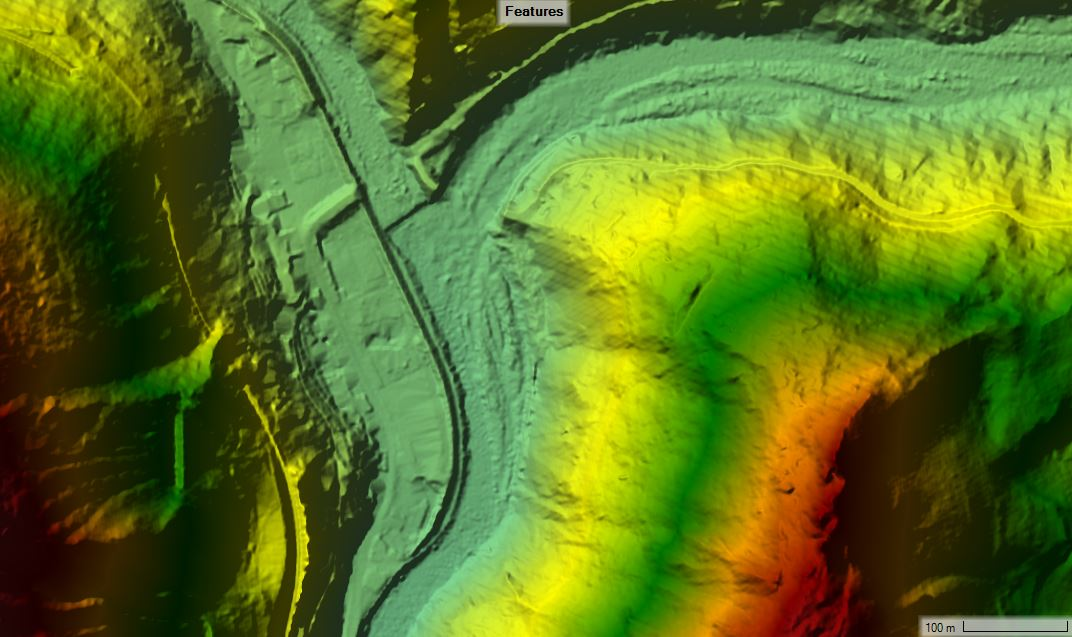
\includegraphics[scale=0.4]{immagini/particolare_dtm.JPG}
    \caption{Particolare del DTM del tratto di studio analizzato.}
    \label{figure:particolare_dtm}
    \end{figure}

Per l'applicazione del modello idraulico, il software utilizza delle equazioni idrauliche, che vanno a considerare, per esempio, le perdite di carico localizzate, continue o le eventuali interazioni tra il flusso d'acqua in movimento e le geometrie dell'alveo \cite{hydraulic_equations}.

\subsection{Geometrie in alveo}
E' molto probabile che, soprattutto in caso di aree altamente urbanizzate, ci siano delle opere idrauliche in alveo, come per esempio soglie o ponti.\\
Affinché il programma ne tenga in considerazione durante il calcolo, è necessario che l'operatore inserisca la geometria del profilo dell'opera, come per esempio del ponte \eqref{figure:profilo_ponte}. 
\begin{figure}[htb] \centering
    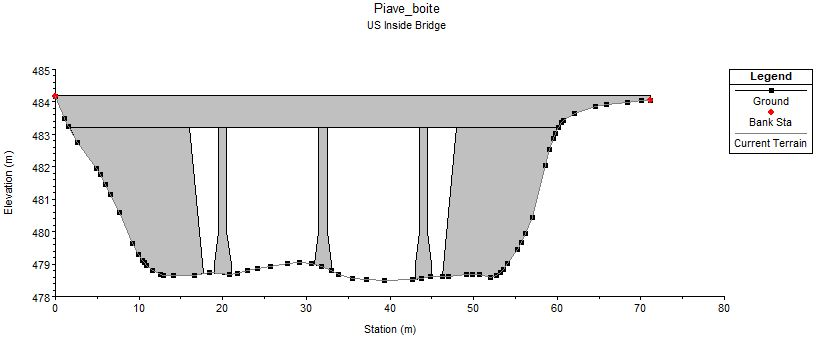
\includegraphics[scale=0.6]{immagini/profilo_ponte.JPG}
    \caption{Profilo di geometria del ponte nel fiume Boite.}
    \label{figure:profilo_ponte}
    \end{figure}
Essendo un corpo che cambia il normale flusso dell'acqua in alveo, HEC-RAS possiede delle proprie equazioni per calcolare il comportamento delle portate \cite{modeling_bridges}.\\
Per quanto riguarda la presenza di soglie, sarebbe opportuno indicarne (mediante breaklines) la presenza, ed eventualmente cambiare il valore di scabrezza nelle celle contenenti la superficie dell'opera (che in molti sono fatte in calcestruzzo).

\subsection{Condizioni al contorno}
Le ``boundary conditions" rappresentano uno dei principali fattori in HEC-RAS, poiché influenzano i volumi e le portate agenti nel processo di simulazione \cite{boundary_conditions}.\\
Le condizioni al contorno sono un insieme di parametri che vanno a descrivere le portate di deflusso in movimento, siano queste entranti o uscenti. Oltre ai semplici valori volumetrici o di portata, è importante riportare la pendenza del thalweg dell'alveo, perché regola la quantità di energia totale.\\
Per il caso di questa relazione, i volumi e le portate sono stati ricavati da una precedente analisi idrologica mediante il software HEC-HMS \cite{progetto_hms}. Comunque, i risultati sono già stati riportati in precedenza all'interno di questa relazione.\\
Per quanto riguarda la pendenza del thalweg, il valore è stato misurato mediante un apposito strumento disponibile all'interno di HEC-RAS. 